\begin{frame}[fragile]{Visualização da remoção de elementos na pilha}

    \begin{figure}[ht]
        \centering
        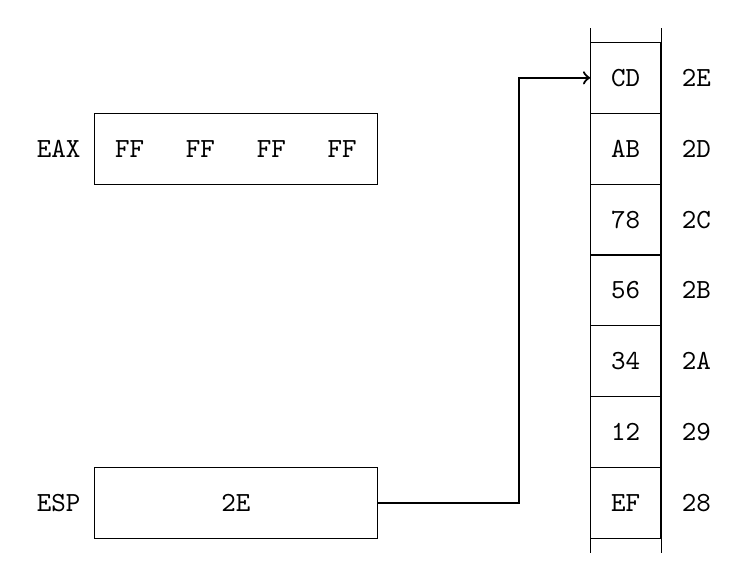
\begin{tikzpicture}[scale=0.9]
            \node at (0.5, 5.5) { \tt FF };
            \node at (1.5, 5.5) { \tt FF };
            \node at (2.5, 5.5) { \tt FF };
            \node at (3.5, 5.5) { \tt FF };
            \node at (-0.5, 5.5) { \tt EAX };
%            \node at (1, 6.5) { \tt AX };
%            \draw (0, 5) rectangle (2, 6);
            \draw (0, 5) rectangle (4, 6);

            \node at (2, 0.5) { \tt 2E };
            \node at (-0.5, 0.5) { \tt ESP };
            \draw (0, 0) rectangle (4, 1);

            \draw (7, 0) grid (8, 7);
            \draw (7, 0) -- (7, -0.2);
            \draw (8, 0) -- (8, -0.2);
            \draw (7, 0) -- (7, 7.2);
            \draw (8, 0) -- (8, 7.2);

            \node at (8.5, 0.5) { \tt 28 };
            \node at (8.5, 1.5) { \tt 29 };
            \node at (8.5, 2.5) { \tt 2A };
            \node at (8.5, 3.5) { \tt 2B };
            \node at (8.5, 4.5) { \tt 2C };
            \node at (8.5, 5.5) { \tt 2D };
            \node at (8.5, 6.5) { \tt 2E };

            \node at (7.5, 0.5) { \tt EF };
            \node at (7.5, 1.5) { \tt 12 };
            \node at (7.5, 2.5) { \tt 34 };
            \node at (7.5, 3.5) { \tt 56 };
            \node at (7.5, 4.5) { \tt 78 };
            \node at (7.5, 5.5) { \tt AB };
            \node at (7.5, 6.5) { \tt CD };

            \draw[->,thick] (4, 0.5) -- (6, 0.5) -- (6, 6.5) -- (7, 6.5);
        \end{tikzpicture}
        \caption{Estado do programa}
    \end{figure}

\end{frame}

\begin{frame}[fragile]{Visualização da remoção de elementos na pilha}

    \begin{figure}[ht]
        \centering
        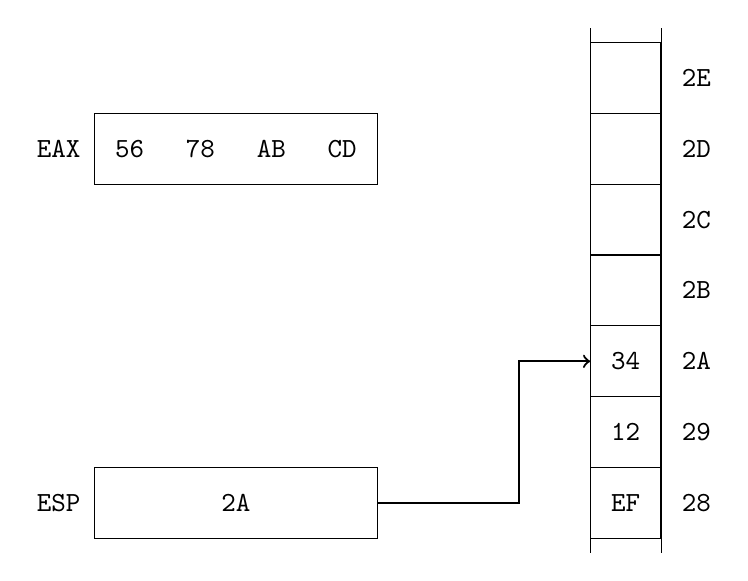
\begin{tikzpicture}[scale=0.9]
            \node at (0.5, 5.5) { \tt 56 };
            \node at (1.5, 5.5) { \tt 78 };
            \node at (2.5, 5.5) { \tt AB };
            \node at (3.5, 5.5) { \tt CD };
            \node at (-0.5, 5.5) { \tt EAX };
%            \node at (1, 6.5) { \tt AX };
%            \draw (0, 5) rectangle (2, 6);
            \draw (0, 5) rectangle (4, 6);

            \node at (2, 0.5) { \tt 2A };
            \node at (-0.5, 0.5) { \tt ESP };
            \draw (0, 0) rectangle (4, 1);

            \draw (7, 0) grid (8, 7);
            \draw (7, 0) -- (7, -0.2);
            \draw (8, 0) -- (8, -0.2);
            \draw (7, 0) -- (7, 7.2);
            \draw (8, 0) -- (8, 7.2);

            \node at (8.5, 0.5) { \tt 28 };
            \node at (8.5, 1.5) { \tt 29 };
            \node at (8.5, 2.5) { \tt 2A };
            \node at (8.5, 3.5) { \tt 2B };
            \node at (8.5, 4.5) { \tt 2C };
            \node at (8.5, 5.5) { \tt 2D };
            \node at (8.5, 6.5) { \tt 2E };

            \node at (7.5, 0.5) { \tt EF };
            \node at (7.5, 1.5) { \tt 12 };
            \node at (7.5, 2.5) { \tt 34 };
%            \node at (7.5, 3.5) { \tt 56 };
%            \node at (7.5, 4.5) { \tt 78 };
%            \node at (7.5, 5.5) { \tt AB };
%            \node at (7.5, 6.5) { \tt CD };

            \draw[->,thick] (4, 0.5) -- (6, 0.5) -- (6, 2.5) -- (7, 2.5);
        \end{tikzpicture}
        \caption{Estado do programa após a instrução \code{nasm}{POP EAX}}
    \end{figure}

\end{frame}

